\documentclass[11pt,a4paper]{article}
\usepackage{graphicx} % Required for inserting images

\usepackage[english]{babel}

\usepackage{geometry}
\usepackage{amsmath}
\usepackage{amssymb}
\usepackage{graphicx}
\usepackage{enumitem}
\usepackage{caption}
\usepackage{subcaption}
\usepackage{indentfirst}
\usepackage[T1]{fontenc}
\usepackage{braket}
\usepackage{hyperref}
\usepackage{fancyhdr,array}
\usepackage[utf8]{inputenc}
\usepackage{csquotes}
\usepackage{makecell}
\usepackage{multirow}
\usepackage[style=numeric,sorting=none]{biblatex}
\addbibresource{bibliography.bib}
\usepackage{wrapfig}
\usepackage{eso-pic} 
\usepackage{dirtree}
\usepackage[version=4]{mhchem}
\usepackage{tabularx}
\usepackage{enumitem}

\usepackage{longtable}

\usepackage{url}

\geometry{top=30mm,bottom=30mm}

% --- Cell setup in tables 
\renewcommand{\cellalign}{tl}
%\renewcommand{\theadalign}{vh}
%\renewcommand{\arraystretch}{5}

% --- Paragraph setup
\frenchspacing  % No double space
\setlength{\parindent}{0mm}     % indent size (start of paragraph)

\setlist{nosep} % removes extra vertical spacing in all lists

\begin{document}

\begin{center}
    \LARGE
    \textbf{HyProC - Manual}

    \Large
    \text{5th November 2026}

    \vspace{0.25cm}
    L. Dupont

    \small
    louis.dupont-2@unamur.be
    
\end{center}

{\setlength{\parskip}{0pt} \tableofcontents}

\setlength{\parskip}{1em}   % spacing between paragraphs

\newpage
\section{Getting started}
From the HyProC folder, run \texttt{UI.py} to launch the application.

Once inside the application, the workflow should be as follows:
\begin{enumerate}
    \item Enter the reaction parameters in the Reaction settings dialog.
    \item Load or create a target.
    \item Load or create a standard, and enter its measured yield. Alternatively, enter a manual $K$ factor.
    \item Adjust the calculation options as needed.
    \item Load an experimental excitation curve.
    \item Hit Run Calculation, this will generate a simulated excitation curve at the experimental energies. Alternatively, manually define an energy range and step size, using the adjacent button.
    \item Use the Chi-squared history graph to evaluate the quality of the simulation and adjust the target and simulation parameters as needed. The Chi-squared values are calculated over the full energy range by default, but can be restricted to a specific energy window using the E Min and E Max fields.
\end{enumerate}

\section{Menu bar}
File:
\vspace{-\parskip}
\begin{itemize}
    \item Load simulation: Restores the target, standard, experimental and simulated curves, calculation options, energy range, and chi-squared history from a HyProC simulation JSON file. Reaction and resonance parameters stored in that file are also written to \texttt{settings.json} and reloaded for subsequent calculations.
    \item Save simulation: Saves the current simulation state to a HyProC simulation JSON file. It includes the current reaction and resonance parameters, and the manual K factor when entered. Target layers are saved as the user-defined layers, not the internal stopping-power segments.
\end{itemize}

Target \& Std:
\vspace{-\parskip}
\begin{itemize}
    \item Load target: Reads a target from a .json file, replacing the current target.
    \item Save target: Saves the current target description to a .json file.

    \item Load standard: Reads a standard from a .json file, replacing the current standard. If the file contains multiple layers, the user selects one layer; the program then uses a fixed standard areal density of 1750 TFU.
    \item Save standard: Saves the current standard description to a .json file.
\end{itemize}

Reaction:
\vspace{-\parskip}
\begin{itemize}
    \item Reaction settings: Opens a dialog for projectile and target atomic and mass numbers ($Z_1$, $A_1$, $Z_2$, $A_2$), and resonance energy, width, and peak cross section ($E_R$, $\Gamma_R$, $\Sigma_R$). The resonance shape is currently fixed to Lorentzian. Confirm saves the values to \texttt{settings.json}; Cancel discards unsaved edits.
\end{itemize}

Plot:
\vspace{-\parskip}
\begin{itemize}
    \item Rescale excitation curve: Resets the excitation plot limits to fit the visible curves.
    \item Autoscale: When on, the excitation plot automatically adjusts its limits after a calculation.
    \item Sim curve markers: Turns markers on or off for the simulated curve.
    \item Chi-squared energy bounds: Shows or hides the current minimum and maximum chi-squared energies on the excitation plot.
    \item Save simulated curve data: Saves the simulated energies and yields in a two-column, tab-separated .txt file.
    \item Load Sim curve as Exp curve: Copies the simulated energies and yields into the experimental curve, with zero uncertainty.
    \item Remove experimental/simulated curve: Removes the corresponding curve from the plot.
    \item Reset Chi-squared history: Clears the recorded chi-squared values.
\end{itemize}

Settings:
\vspace{-\parskip}
\begin{itemize}
    \item Settings: Opens a window to set the SRIM folder, data-save folder, and expected column names for imported excitation curves.
    \item Manual: Opens this manual in the system's default PDF viewer.
\end{itemize}

\section{Main window}
The main window is arranged as a control panel on the left, a Target/Standard editor in the centre, and the excitation-curve plot below. The menu bar provides additional file, plot, and settings commands described in the previous section.

\subsection{Curve input and calculation}
\paragraph{Import excitation curve}
Select an Excel workbook (\texttt{.xlsx}, \texttt{.xls}), CSV file (\texttt{.csv}), or delimited text file (\texttt{.txt}) to load experimental data. HyProC looks for the configured energy and yield column names; the uncertainty column is optional and is set to zero when absent. CSV and text files can also be read as two or three columns (energy, yield, and optionally uncertainty). The expected column names can be changed in Settings. If a workbook contains multiple matching sheets or tables, HyProC asks which one to import. Imported points are ordered by energy.

\paragraph{Run Calculation}
The main button uses the existing simulated energy values when available. If there is no simulated curve, it uses the loaded experimental energies; if neither exists, it opens the energy-range dialog. Use the adjacent arrow to choose among the normal calculation, a custom energy range, and the loaded experimental-curve energies. A custom range is entered as minimum energy, maximum energy, and step size in keV. If the final step does not land exactly on the maximum, that maximum is included as the final point. The energy offset is subtracted before calculation and added back to the energies displayed in the plot.

After a successful calculation, the simulated curve is plotted and the elapsed calculation time is printed to the console. If an experimental curve is loaded, HyProC also records a chi-squared-history value using the currently selected energy bounds.

\paragraph{Extract profile}
Opens a separate plot of the hydrogen depth profile derived from the current target.

\subsection{Standard and K factor}
The Standard panel contains an optional manual K factor, the measured standard yield in Counts/$\mu$C, and Load/Save buttons for the standard. Entering a positive manual K factor bypasses the standard-based K calculation and disables the standard controls. 

Without a manual K factor, load a standard and enter its measured yield. A standard should be uniform; if the JSON file contains multiple layers, HyProC asks which layer to retain. The standard is treated as one layer with a fixed areal density of 1750 TFU. Its yield is evaluated at $E_R+100\,\Gamma_R$ when calculating K. 

See section~\ref{sec:efficiency} for details on the $K$ factor and standard.

\subsection{Calculation options}
The Options panel controls the physical models and output:
\begin{itemize}
    \item \textbf{Stopping model:} SCS-25-Solid (the default) or SRIM (see section \ref{sec:stopping}).
    \item \textbf{Straggling model:} None, Rud, Rud corr (the default), or Bohr.
    \item \textbf{Beam width SD (keV):} Standard deviation of the incident ion beam energy distribution (assumed to be gaussian). If set to 0, the beam is considered mono-energetic.
    \item \textbf{Offset (keV):} Energy offset used for the calculation and reversed for displayed curve energies.
    \item \textbf{Quantum Doppler:} Includes or omits the quantum Doppler contribution.
    \item \textbf{Save broadening data:} Writes intermediate broadening data for each calculation run. The output folder structure is described in the Broadening data subsection.
    \item \textbf{Track target changes:} Saves a copy of the target used for each calculation run.
\end{itemize}

\subsection{Target and standard editor}
Use the Target and Standard tabs in the central editor to select which composition to edit. The target editor has a Layers list on the left and an Elements list on the right. Selecting a layer displays its areal density in TFU; selecting an element displays its atomic number $Z$ and atomic percentage. Edit these values directly and press Enter or leave the field to apply the change.

The target's layer controls add or remove a layer, move the selected layer up or down, and duplicate it. The element controls add or remove an element from the selected layer. \textbf{Isolate \& Normalize} keeps the selected element's percentage fixed and proportionally adjusts the other elements so the layer totals 100\%. The lists retain their scroll position when refreshed, and newly added layers or elements are brought into view.

The Standard tab has the same element-composition list, editable $Z$ and atomic-percentage fields, and Add Element, Remove Element, and Isolate \& Normalize controls. Standard thickness is fixed by the application; there are no standard layer controls.

\subsection{Excitation-curve plot}
The plot distinguishes experimental data (blue points with uncertainty bars) from the simulated curve (an orange dashed line). The Matplotlib toolbar below the plot provides its usual navigation and image-saving tools. Use the Plot menu to rescale the view, toggle automatic rescaling after calculations, show or hide simulated-curve markers and chi-squared energy-bound lines, save simulated values as a tab-separated text file, copy the simulation into the experimental curve, remove either curve, or reset the chi-squared history.

\subsection{Chi-squared history}
The Chi-squared history panel shows up to nine calculation results at a time. Use Scroll Up and Scroll Down to navigate older and newer results. Enter optional inclusive E Min and E Max bounds in keV to restrict the experimental points used for the next comparison; either bound can be left blank. The excitation plot can display the selected bounds as vertical lines. Blue history bars used the current bounds, while gray bars were calculated with different bounds. The statistic shown is an unweighted mean squared residual, as detailed in the Results subsection.

\section{Physics}
\subsection{Stopping cross-section/power}
\label{sec:stopping}
Note: Stopping cross-section and stopping power describe the same physical property but in 2 different manners. Stopping cross-section is expressed in eV/TFU\footnote{1 TFU (Thin Film Units) = $10^{15}\, \text{at.}/\text{cm}^2$ } whilst stopping powers are in eV/nm thus requiring knowledge of the material's density.

HyProC represents stopping as constant within each calculation-target layer. For the first layer, the incident energy $E_0^\text{In}$ is the minimum energy in the range used for the simulation. The projectile species comes from the Reaction settings. The energy at the layer exit is estimated as:
\begin{equation}
    E_0^\text{Out}[\text{keV}] = E_0^\text{In} - S(E_0^\text{In})\, x
\end{equation}
where $x$ is the layer areal density in TFU. The code calculates stopping at both layer boundaries and compares them using the relative difference:
\begin{equation}
    \frac{|S_\mathrm{in}-S_\mathrm{out}|}
    {\max(|S_\mathrm{in}|,|S_\mathrm{out}|)}.
    \label{eq:stoppingVariation}
\end{equation}
If it exceeds 0.5\%, the layer is subdivided into twice as many equal segments and the check is repeated. Each calculation segment is assigned the mean boundary stopping:
\begin{equation}
    S[\text{keV/TFU}] = \frac{1}{2}
    \left(S(E_0^\text{Out}) + S(E_0^\text{In})\right).
    \label{eq:S_mid}
\end{equation}
The check and stopping assignment are then performed sequentially through the target. Segmentation is internal: the target editor and target/simulation files continue to use the original user-defined layers.

The default model is SCS-25-Solid \cite{meersschaut2026flexible}. It calculates electronic stopping using the tabulated SCS-25-Solid parametrization from Meersschaut \textit{et al.} and adds universal Ziegler nuclear stopping. In compounds, electronic and nuclear components are each combined using the atomic fractions (Bragg addition). The incident energy is converted to energy per projectile mass unit for the electronic parametrization. SRIM \cite{ziegler2010srim} is available as an alternative and requires a valid SRIM path in Settings.

\subsection{Quantum Doppler}
This option includes a Gaussian Doppler contribution associated with hydrogen bound in the target matrix. The implementation uses values for Si, Ti, and Pb matrices and an effective-atomic-number fit for other matrices; compounds use a Bragg-rule effective value. The checkbox in Options switches this contribution on or off.

Hydrogen is usually well localized in chemical bonds. The resulting uncertainty in momentum and velocity causes a Gaussian broadening of the reaction resonance, known as the quantum Doppler effect \cite{horn1988observation}. Its standard deviation can be expressed as:
\begin{equation}
    \delta_D[\text{keV}] = \sqrt{\cfrac{2 m_1 E_H E_R}{m_H}}
    \label{eq:dopplerSD}
\end{equation}
where $m_1$, $m_H$, $E_H$ and $E_R$ are the projectile and hydrogen masses, the hydrogen zero-point vibrational energy, and the resonance energy, respectively. In the implementation, literature-based values are used for Si, Ti, and Pb matrices. For other matrices, the following fit is used:
\begin{equation}
    \delta_D[\text{keV}] = -0.0218\,Z + 4.24
    \label{eq:dopplerSDfit}
\end{equation}
where $Z$ is the effective atomic number of the matrix (using a Bragg rule for compounds). The matrix-specific implementation is an approximation to the physical relation above.

\subsection{Straggling}
Statistical variations in the number of collisions between the projectiles and the target's electrons lead to a broadening of the energy distribution of the beam as it penetrates the target. To describe this, HyProC considers a gaussian broadening whose standard deviation $\delta_S$ can be obtained using different models:
\paragraph{None}
No energy straggling is included ($\delta_S=0$).
\paragraph{Rud}
This empirical formula was developed by Rud for a \ce{^15N} beam \cite{rud1978measurements}:
\begin{equation}
    \delta_S(x)[\text{keV}] = \cfrac{2.03}{2.355}\, Z_2^{0.39} \sqrt{x}
    \label{eq:straggSD_Rud}
\end{equation}
where $Z_2$ is the atomic number of the material and $x$ its areal density in units of $10^{16} \text{ at./cm}^2$.
\paragraph{Rud corr (corrected)}
During testing of Rud's model, straggling was found to be overestimated. Results obtained using the Rud formula were then compared with SRIM outputs, revealing a discrepancy factor of 1.7. A second straggling model "Rud corr" was thus implemented in HyProC:
\begin{equation}
    \delta_S(x)[\text{keV}] = \cfrac{1}{1.7}\, \cfrac{2.03}{2.355}\, Z_2^{0.39} \sqrt{x}
    \label{eq:straggSD_Rudcorr}
\end{equation}
Bohr's straggling model is also implemented \cite{bohr1948penetration}:
\begin{equation}
    \delta_S(x)[\text{keV}] = \sqrt{0.260532\ Z_1^2 Z_2 x}
    \label{eq:straggSD_Bohr}
\end{equation}
with $x$ in $10^{18} \text{ at./cm}^2$

For compounds, HyProC calculates straggling separately for each element, weights each variance by that element's atomic fraction, and sums the variances. For instance \cite{wang2010handbook}:
\begin{equation}
    \delta_{\ce{SiO_2}}^2(x)[\text{keV}^2] = \frac{1}{3} \, \delta_{\ce{Si}}(x)^2 + \frac{2}{3}\, \delta_{\ce{O}}(x)^2
\end{equation}
Note that for small energy loss and thin layers, the straggling isn't gaussian. The distribution is asymmetric and follows Vavilov's theory \cite{vavilov1957ionization}. This is currently NOT implemented in HyProC.

\section{Calculations}

\subsection{Excitation curve and broadenings}
HyProC calculates the excitation curve for a given target and incident energy range. The yield $Y(E_i)$ (expressed in Counts/µC) at each incident energy $E_i$ is obtained by integrating the product of the instrument function $F(E,E_i,x)$ and the hydrogen depth profile $n_\text{H}(x)$ over the target depth:
\begin{equation}
    Y(E_i) = K \int_{0}^{\infty} F(E,E_i,x) \, n_\text{H}(x)\, dx
    \label{eq:yield}
\end{equation}
with 
\begin{equation}
    F(E, E_i, x) =  \sigma(E) \ast B(E,E_i) \ast D(E) \ast S(E,x)
\end{equation}
where $\sigma(E)$ is the resonance cross-section, $B(E,E_i)$ is the beam width, $D(E)$ is the Quantum Doppler broadening, and $S(E,x)$ is the straggling broadening. The symbol $\ast$ denotes convolution. The cross section is assumed to have a Lorentzian shape:  
\begin{equation}
    \sigma(E) =
    \sigma_R\,
    \frac{\Gamma_R^2/4}
    {(E-E_R)^2+\Gamma_R^2/4},
\end{equation}
where $E_R$ is the resonance energy, $\Gamma_R$ is the resonance width and $\sigma_R$ is the resonance intensity. The beam width, Doppler, and straggling contributions are treated as independent Gaussian:
\begin{equation}
    G(E) =
    \frac{1}{\sqrt{2\pi}\,\delta_G}
    \exp\left[-\frac{(E-E_c)^2}{2\delta_G^2}\right].
\end{equation}
$K$ is a constant representing the efficiency of the experimental system, including the intrinsic efficiency of the detector and its solid angle. See section~\ref{sec:efficiency} for details.

For each incident energy, HyProC first uses the stopping cross-sections and areal densities of the target layers to determine the energy loss through the target, the layer and the depth at which the nominal resonance energy $E_R$ is reached. Based on that, the program calculates the energy straggling of the ion beam as well as the quantum Doppler contributions, based on the models described in the previous sections. Those contributions are combined with the user-specified beam width to form a total Gaussian broadening:
\begin{equation}
    \delta_\text{Gauss} = \sqrt{\delta_B^2 + \delta_S^2 + \delta_D^2}.
\end{equation}
The program then convolves this Gaussian with the Lorentzian resonance cross-section to obtain a Voigt-shaped profile. This profile is then mapped from energy to areal depth (using stopping cross-sections), yielding the instrument function $F(E,E_i,x)$ used in equation~\ref{eq:yield}. This process can be visually followed in Figure~\ref{fig:combined}.

\begin{figure}[h!]
    \centering
    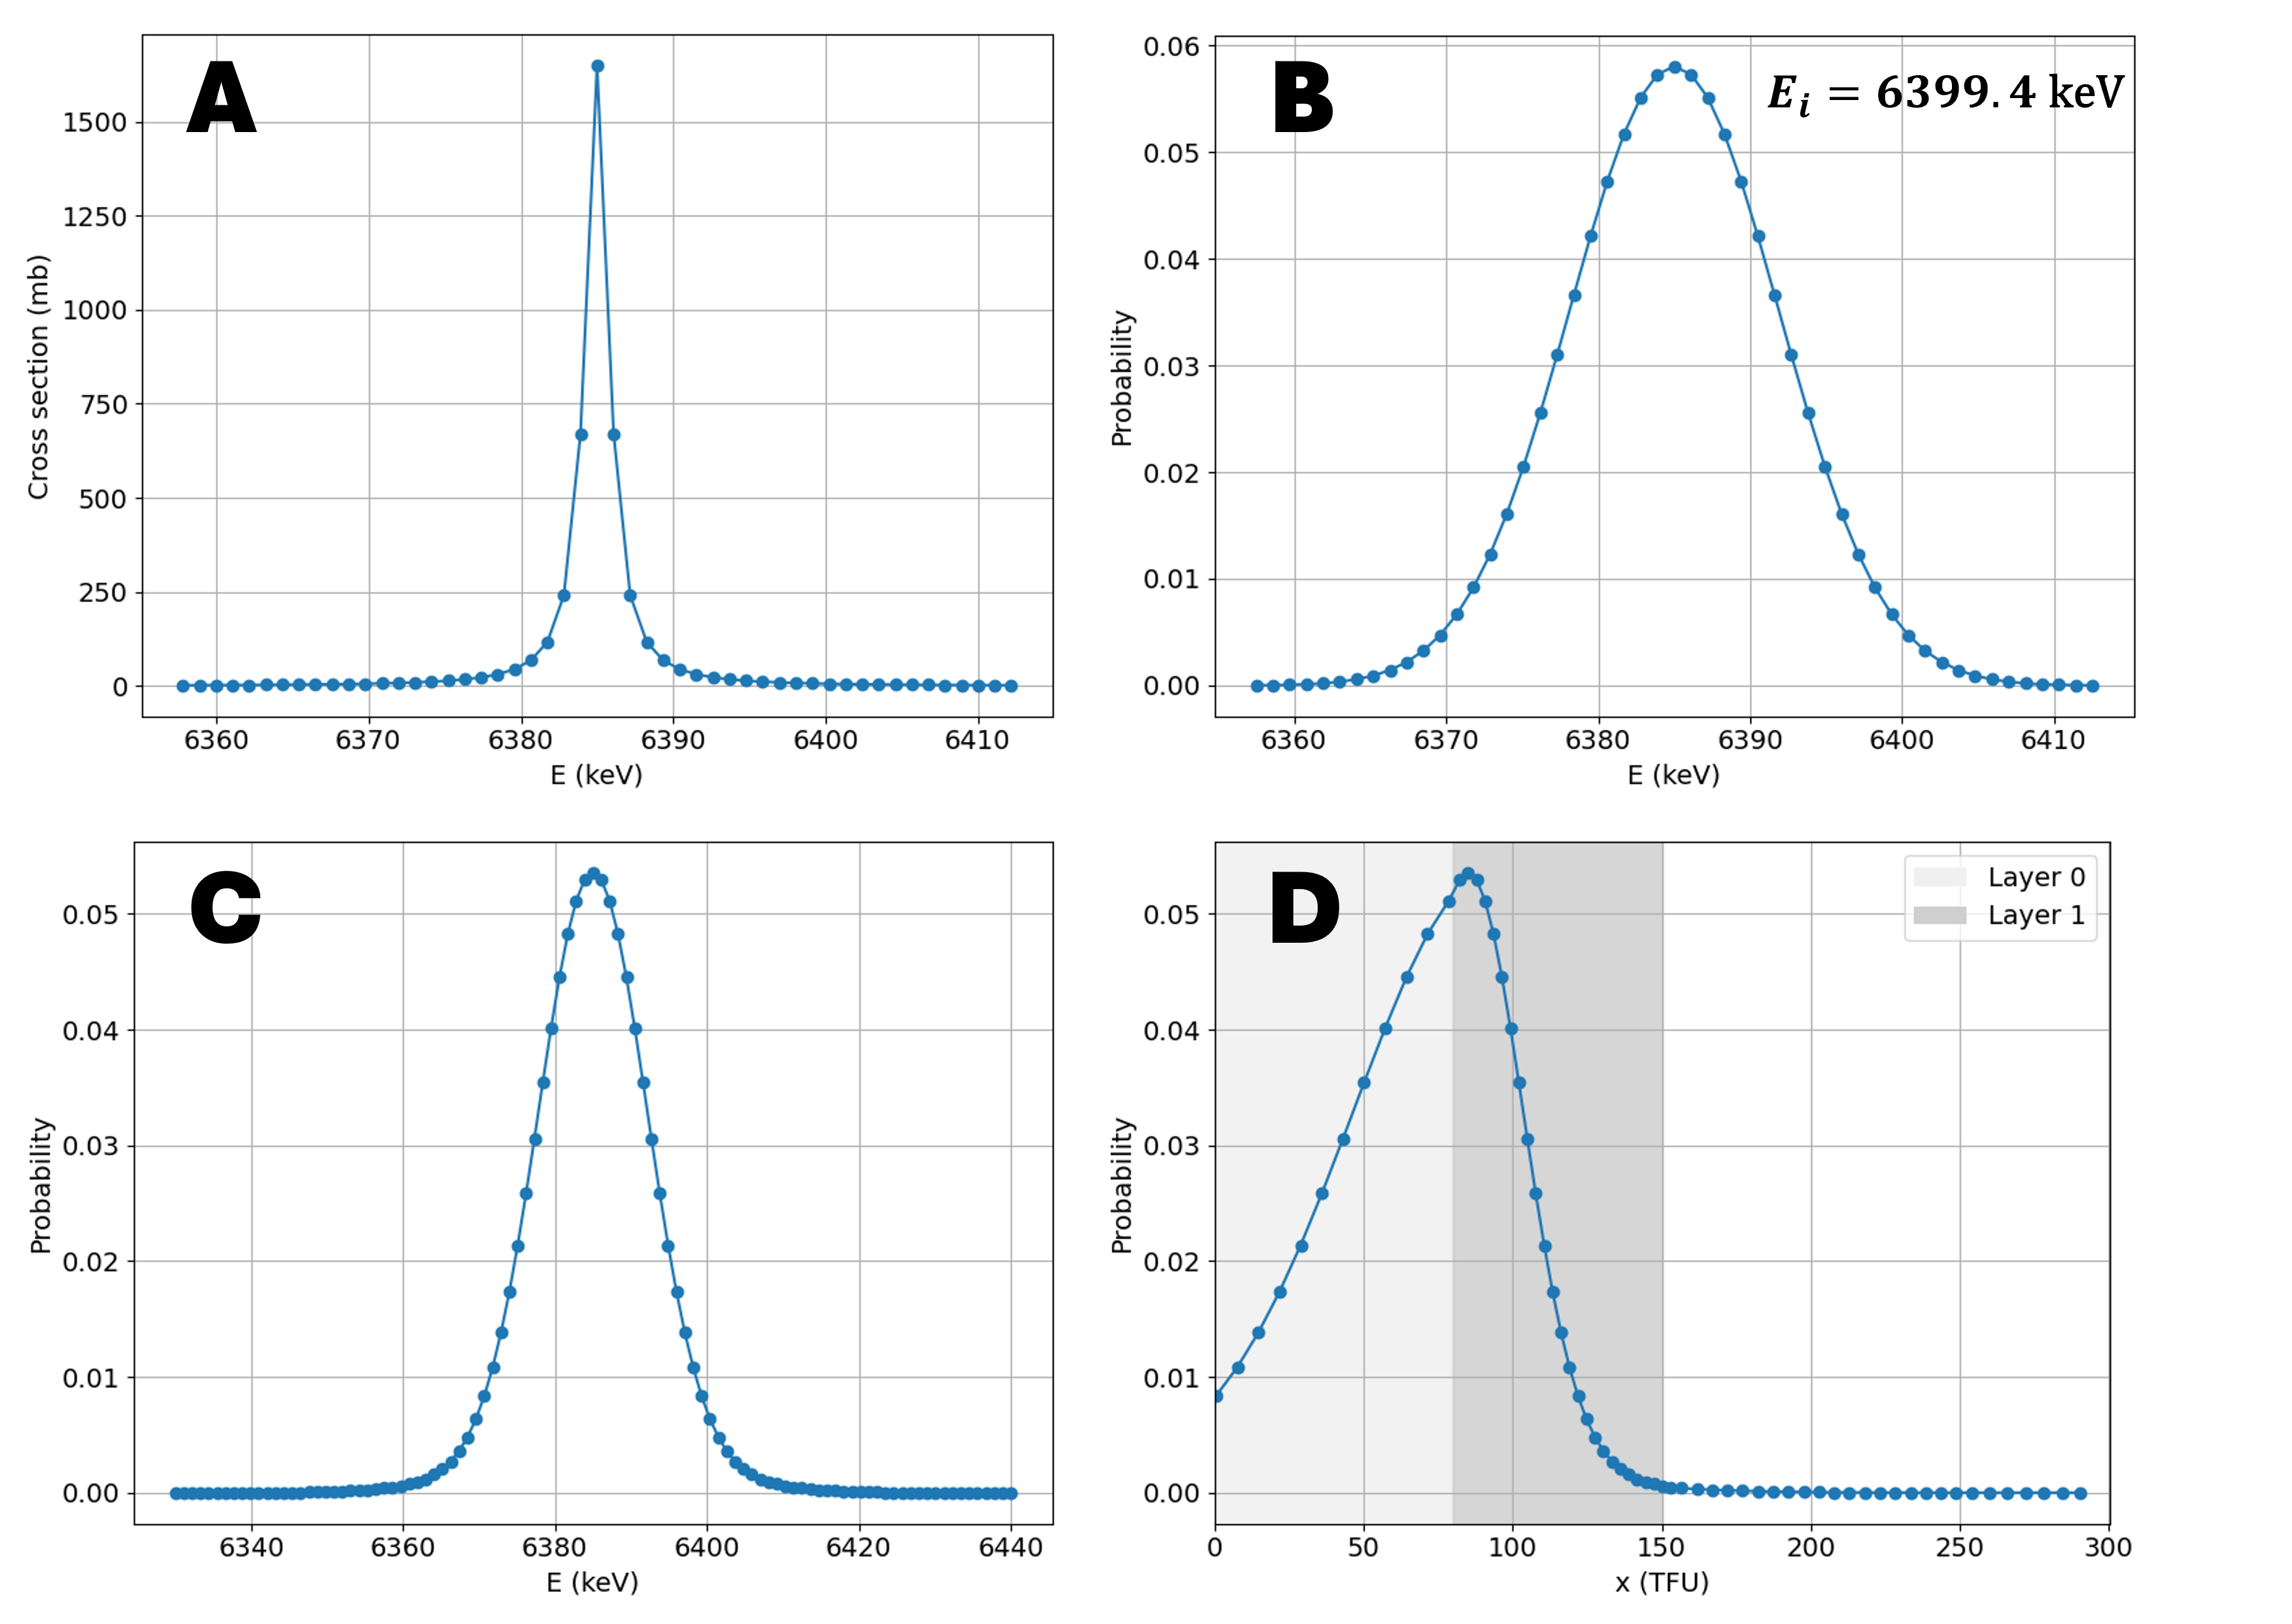
\includegraphics[width=15.5cm]{figures/Combined v2.png}
    \captionsetup{margin=1cm}
    \caption{Example broadening profiles for a 6399.4 keV \ce{^15N} beam impinging on a two-layer target: 80 TFU of \ce{C_{0.83}H_{0.17}} ($S_0=0.155$ keV/TFU) over 75 TFU of \ce{Si_{0.86}H_{0.14}} ($S_1=0.392$ keV/TFU). (A) Lorentzian resonance cross-section, (B) combined Gaussian broadening from beam width, straggling, and Doppler motion, (C) convolution of A and B, and (D) profile from C mapped onto areal depth in TFU.}
    \label{fig:combined}
\end{figure}

Broadening data can be saved by ticking the "Save broadening data" box. When calculations are made  with this option on, folders will be created using this architecture:

\dirtree{%
.1 HyProC save path/.
.2 Session/.
.3 Run/.
.4 Datapoint/.
.5 Beam.txt.
.5 Stragg.txt.
.5 Doppler.txt.
.5 Total\_Gauss.txt.
.5 xsec.txt.
.5 Total\_Broadening.txt.
.5 Total\_Broadening\_TFU.txt.
}

\texttt{Total\_Gauss.txt} contains the combined Gaussian from beam width, straggling, and (when enabled) Doppler broadening. \texttt{xsec.txt} contains the Lorentzian resonance cross-section. Their convolution is saved as \texttt{Total\_Broadening.txt}; this is the energy-axis profile shown in Figure~\ref{fig:combined}(C). \texttt{Total\_Broadening\_TFU.txt} contains the corresponding profile mapped to areal depth in TFU, as in Figure~\ref{fig:combined}(D). The separate \texttt{Beam.txt}, \texttt{Stragg.txt}, and \texttt{Doppler.txt} files show the individual Gaussian components used to form the total Gaussian.

A Session folder is created when broadening data are saved or that the track target changes option is enabled for the first time after the UI is launched. A Run folder is created whenever a calculation is made (with the save broadening data on or with the target tracking on). For each incident energy, a datapoint folder is created.

The broadening data can be visualised using the broadplotter.py script (recommended) or through a third-party software (OriginLab, ...).

\subsection{Standard/CRM}
\label{sec:efficiency}
The constant $K$ in equation (\ref{eq:yield}) represents the efficiency of the experimental system which includes the intrinsic efficiency of the detector as well as its solid angle.

It is on paper possible to obtain those two quantities to calculate $K$, but it is quite challenging in practice. To circumvent this issue, a measurement is made on a standard sample, also called CRM (Certified Reference Material). It is a sample whose composition is stable under irradiation, depth-uniform and very accurately known. This allows to invert equation (\ref{eq:yield}) and obtain a value for $K$:
\begin{equation}
    K = Y^\text{std}(E_i)\ / \int_{0}^{\infty} F^\text{std}(E,E_i,x) \, n_H^\text{std}(x)\, dx
\end{equation}
which then can be plugged back into equation (\ref{eq:yield}) for a sample of interest.

The standard has the same layer and composition format as the target but is treated as a single layer with a fixed areal density of 1750 TFU (not editable in the UI).

When using a standard to calculate $K$, the program evaluates the integral at an incident energy of
\[
    E_i = E_R + 100\,\Gamma_R,
\]
with energies in keV. Enter the measured standard yield at this energy in the Standard panel; exclude any non-resonant background. Alternatively, the user can manually enter a positive manual $K$ factor in the $K$ factor field, disabling standard inputs and controls and skipping the $K$ calculation.

\subsection{Results: Chi-square test}
When a simulated excitation curve is generated, the program compares it with the experimental curve over the selected energy bounds. The simulated yields are interpolated at the experimental energies where necessary. The value displayed in the "Chi-squared history" graph is the mean squared residual (called chi-squared by the application):
\begin{equation*}
\chi^2 =
\cfrac{1}{N}\ \sum\limits_{i=1}^{N} (y_{\mathrm{exp},i} - y_{\mathrm{sim},i})^2
\end{equation*}
where $N$ is the number of valid overlapping experimental points. This is an unweighted mean squared difference; experimental uncertainties are not used in this statistic. E Min and E Max in the Chi-squared history panel set the inclusive energy range. The excitation plot can show these bounds, and the history bars are blue when their recorded bounds match the currently selected bounds and gray otherwise.

%\begin{figure}[t!]
%    \centering
%    \includegraphics[width=8cm]{graph_acc.png}
%    \captionsetup{justification=centering,margin=3cm}
%    \caption{Graphique de la précision d'entraînement et de test en fonction de la valeur de \textit{max\_depth}.} 
%    \label{fig:graph_acc}
%\end{figure}

\clearpage
\printbibliography[heading=bibintoc]

\end{document}
